\documentclass[DIV=calc, paper=a4, fontsize=11pt, twocolumn]{scrartcl}
\usepackage{microMathematics-de}
\usepackage[english,german]{babel}

% Begin document
\begin{document}
\maketitle
\thispagestyle{fancy} % Enabling the custom headers/footers for the first page

\begin{bf}
% This is the first part of the file about_micromath_de.tex
Der microMathematics Plus ist der erste
mathematische Taschenrechner für
Android weltweit, der auf einer
Kalkulationstabelle basiert, welche es
erlaubt, mathematische Elemente live
einzugeben und zudem hochgenaue
Berechnungen liefert.

Diese App basiert auf einem
leistungsstarken Touchscreen Editor,
der alle grundlegenden mathematischen
Bezeichnungen beinhaltet und Nutzern
erlaubt, ganz selbstverständlich
lesbare Arbeitsblätter zu erstellen
und zu bearbeiten.

Der microMathematics Plus unterstützt
nur mathematische Berechnungen auf
Sekundarstufenniveau. Diese Version
hat folgende Einschränkungen: sie
unterstützt weder Sonderfunktionen,
Vektoren, Matrizen noch viele andere
Dinge auf mathematisch höherem Niveau.
\end{bf}

\section{Benutzung}
% This is auto-generated file: do not edit!
% Exported from microMathematics Plus, version 2.15.3


Diese App ist eine leistungsstarke
Rechensoftware im Arbeitsblatt Format.
Das Arbeitsblatt kann frei editiert,
auf einer SD Karte gespeichert werden,
von einer SD Karte aus geöffnet oder
in ein Bild- oder LaTeX-Format
exportiert werden. Es ermöglicht die
sofortige Bearbeitung von eingesetzten
mathematischen Bezeichnungen sowie
deren automatische Berechnung.

Die folgenden Objekte stehen zur
Verfügung: Gleichungen,
Ergebnisansichten, graphische
Darstellungen, Textfragmente und
Bilder. Diese Broschüre gibt Ihnen
einen Überblick darüber, wie man diese
Objekte erstellen und bearbeiten kann.

\subsection{Bearbeitung}

Fast alle Objekte bestehen aus frei
editierbaren Feldern. Um das Feld zu
bearbeiten, nutzen Sie die Symbole und
Funktionen der Werkzeugleiste.

Alle Symbole können auch über die
Tastatur eingefügt werden. Um
herauszufinden, welche Taste mit
welchem mathematischen Symbol
korrespondiert, lesen Sie den Hinweis
indem Sie den jeweiligen Button lange
gedrückt halten.

Langes Gedrückthalten eines Terms
erlaubt Ihnen, diesen Term
auszuwählen. Der ausgewählte Term kann
gelöscht, in die Zwischenablage
kopiert, von dort aus eingefügt
werden, oder eine Funktion oder ein
Symbol kann im Nachhinein von der
Werkzeugleiste oder Tastatur aus
eingefügt werden.

Sie können auch den ''Rückgängig''
Button in der Menüleiste benutzen, um
die letzte Eingabe rückgängig zu
machen:
\begin{center}\begin{tabular}{c} 
\includegraphics[resolution=320]{how_to_use_fig1.png} \end{tabular}\end{center}

\subsection{Gleichungen}

Eine Gleichung definiert eine
numerische Konstante, ein Intervall
oder eine Funktion. Um eine Gleichung
zu erstellen, nutzen Sie den ''Neu''
Button in der Menüleiste
\begin{center}\begin{tabular}{c} 
\includegraphics[resolution=320]{how_to_use_fig2.png} \end{tabular}\end{center}

oder den ''Gleichung hinzufügen'' Button
der Werkzeugleiste:
\begin{center}\begin{tabular}{c} 
\includegraphics[resolution=320]{how_to_use_fig3.png} \end{tabular}\end{center}

Eine Gleichung mit zwei lehren Feldern
wird erstellt:
\begin{center}\begin{tabular}{c}
  ${\Box} := {\Box}$
\end{tabular}\end{center}

Der Name der Gleichung muss in dem
linken Feld eingegeben sein. Der Name
darf nur Buchstaben und Zahlen
enthalten und wird in anderen
Gleichungen genutzt, um auf diese
Gleichung zu verweisen.

Sie können Menüleiste benutzen, um
''Dokumenteinstellungen'' Dialog zu
öffnen:
\begin{center}\begin{tabular}{c} 
\includegraphics[resolution=320]{how_to_use_fig4.png} \end{tabular}\end{center}

Abhängig vom Parameter ''Neubestimmung
erlauben'' in diesem Dialog sind zwei
Benutzungsmodi möglich:

a) Falls eine Neubestimmung nicht
erlaubt ist, bleibt die Gleichung
einzigartig im gesamten Arbeitsblatt
und die Gleichung kann sowohl vor als
auch nach ihrer Bestimmung verwendet
werden.

b) Falls eine Neubestimmung erlaubt
ist, können Sie mehr als eine
Gleichung mit dem selben Namen
bestimmen. Falls so eine Gleichung
dann referenziert wird, verwendet die
Software die zuletzt bestimmte
Version.

\subsubsection{Konstanten}

Falls der Name der Gleichung keine
Parameter in Klammern enthält,
definiert diese eine Konstante oder
ein Intervall:
\begin{center}\begin{tabular}{ccc}
  $N := 200$ &
  $Sq2 := \sqrt{100} $ &
  $Pi2 := \frac{{\pi}}{2}$ \cr
\end{tabular}\end{center}

In diesem Beispiel wurde die
integrierte Konstante Pi verwendet.
Aktuell sind folgende integrierte
Konstanten verfügbar: 
\begin{center}\begin{tabular}{ccc}
  ${\pi} = 3.14159$ &
  $pi = 3.14159$ &
  $e = 2.71828$ \cr
\end{tabular}\end{center}

Es kann auch eine zuvor definierte
Konstante verwendet werden: 
\begin{center}\begin{tabular}{c}
  $NPi2 := N \cdot Pi2$
\end{tabular}\end{center}

Eine komplexe Zahl als eine Konstante
wird durch zwei reele Zahlen und
imaginäre Einheit ''i'' definiert:
\begin{center}\begin{tabular}{c}
  $z := 5+3i$
\end{tabular}\end{center}

\subsubsection{Intervalle}

Eine Intervall-Gleichung definiert
eine Variable, die sich von einem
vorgegebenen Minimalwert in einem
vorgegebenem Schritte zu einem
vorgegebenen Maximalwert verändert.
Diese Variable kann als Parameter
genutzt werden, um eine
Funktionswert-Tabelle oder einen
Funktionsgraphen zu erstellen.

Um ein Intervall zu definieren, legen
Sie einen Namen auf der linken Seite
einer leeren Gleichung fest. Wählen
Sie auf der rechten Seite der
Gleichung entweder das Symbol '':'' oder
klicken Sie den Button ''Äquidistantes
Intervall'' in der Werkzeugleiste:
\begin{center}\begin{tabular}{c} 
\includegraphics[resolution=320]{how_to_use_fig5.png} \end{tabular}\end{center}

Das erste Element ist hier der
Anfangspunkt des Intervalls; das
nächste ist der zweite Punkt und das
letzte Element ist der Endpunkt des
Intervalls.
\begin{center}\begin{tabular}{c}
  $x := \left[ 0,\, 0.1 \,..\, 10 \right]$
\end{tabular}\end{center}

Man kann auf die Intervallemente
zugreiffen:
\begin{center}\begin{tabular}{ccc}
  $x \left( 0\right)  = 0.0$ &
  $x \left( 1\right)  = 0.1$ &
  $x \left( 100\right)  = 10.0$ \cr
\end{tabular}\end{center}

Der Abstand ist hier als Unterschied
zwischen dem zweiten und dem ersten
Wert gegeben:
\begin{center}\begin{tabular}{c}
  $x \left( 1\right)  - x \left( 0\right)  = 0.1$
\end{tabular}\end{center}

Beispielsweise können wir ein
äquidistantes Intervall definieren,
das bei Null beginnt und N Punkte mit
einem Abstand von ''dy'' hat:
\begin{center}\begin{tabular}{cc}
  $dy := 0.05$ &
  $y := \left[ 0,\, dy \,..\, dy \cdot \left( N - 1 \right) \right]$ \cr
\end{tabular}\end{center}

\subsubsection{Funktionen}

Eine Funktion ist eine Beziehung
zwischen zwei Mengen, die jedem
Element oder Wert der einen Menge
genau ein Element der anderen Menge
zuordnet.

Der Funktionsname und das
Funktionsargument in Klammern sind
links von der Gleichung zu finden. Das
Argument muss nicht zuvor im
Arbeitsblatt definiert worden sein.
Sie können es nach Belieben unter
Verwendung von Buchstaben und Zahlen
definieren:
\begin{center}\begin{tabular}{c}
  $f(t) := sin \left( t\right)  \cdot cos \left( t\right)  / 2$
\end{tabular}\end{center}
\begin{center}\begin{tabular}{c}
  $w(z) := {e}^{2i \cdot {\pi} \cdot z}$
\end{tabular}\end{center}
\begin{center}\begin{tabular}{c}
  $g(x,y) := \frac{sin \left( hypot \left( x,\, y\right) \right) }{hypot \left( x,\, y / 2\right)  + 1}$
\end{tabular}\end{center}

Rechts von der Funktion findet sich
eine mathematische Formel um die
Funktion zu berechnen. Falls diese
Formel das Funktionsargument nicht
enthält, wird diese Funktion als
Konstante interpretiert.

Sie können also in dieser Formel eine
integrierte oder zuvor definierte
Funktion einzufügen. Geben Sie dafür
einen Namen ein, klicken Sie auf das
linke Klammer-Symbol ''('' und wählen
Sie das Argument. Dies kann auch eine
Formel sein, die andere Operatoren
oder Funktionen enthält.

\subsubsection{Array}

Arrays sind besondere Funktionen, die
folgende Eigenschaften haben:

a) jedes Argument des Arrays muss ein
vorher definiertes Intervall sein:
\begin{center}\begin{tabular}{cc}
  $k := \left[ 0,\, 1 \,..\, 100 \right]$ &
  $m := \left[ 0,\, 1 \,..\, 200 \right]$ \cr
\end{tabular}\end{center}

a) die Argumente des Arrays sind in eckigen
Klammern ''[ ]'' anstelle der runden
Klammern ''( )'' geschrieben:
\begin{center}\begin{tabular}{c}
  $M[k,m] := {sin \left( k / 10\right) }^{2} - 3 \cdot  \left| cos \left( m / 10\right)  \right| $
\end{tabular}\end{center}

c) die Array-Elemente werden berechnet
und gespeichert. Dadurch ist der
Zugriff auf diese Elemente viel
schneller.

d) man kann die Array-Elemente nur
mittels eines Index zugreifen. Um
solchen Index zu erzeugen, geben Sie
''['' nach dem Array-Namen:
\begin{center}\begin{tabular}{cc}
  $M_{5,\, 10}  = -1.39106$ &
  $M_{10,\, 5}  = -1.92467$ \cr
\end{tabular}\end{center}

e) wenn ein Index ist komplex, negativ 
oder größer als die Obergrenze des
dazugehörigen Intervalls, dann wird
ein ungültigen Wert zurückgegeben:
\begin{center}\begin{tabular}{cc}
  $M_{10i,\, 100}  = NaN$ &
  $M_{90,\, 210}  = NaN$ \cr
\end{tabular}\end{center}

\subsection{Ergebnisansicht}

Dieses Element soll das Ergebnis einer
Berechnung als Zahl oder Tabelle
darstellen. Um eine Ergebnisansicht zu
erstellen, verwenden Sie den ''Neu''
Button in der Menüleiste oder
''Ergebnisansicht hinzufügen'' Button in
der Werkzeugleiste:
\begin{center}\begin{tabular}{c} 
\includegraphics[resolution=320]{how_to_use_fig6.png} \end{tabular}\end{center}

Eine Gleichung mit zwei lehren Feldern
wird erstellt:
\begin{center}\begin{tabular}{c}
  ${\Box} = {\Box}$
\end{tabular}\end{center}

Der linke Term enthält eine zu
berechnende Formel und der rechte Term
ist das Rechnungsergebnis. Hier können
Sie sämtliche zuvor bestimmten
Konstanten und Funktionen verwenden,
sowie alle integrierte Funktionen:
\begin{center}\begin{tabular}{c}
  ${e}^{{\pi}} \cdot f \left( NPi2\right)  = 2.27286E-14$
\end{tabular}\end{center}

Falls der linke Teil keine
''intervallähnlichen'' Variablen enthält
ist das Rechenergebnis nur eine reelle
oder komplexe Zahl.
\begin{center}\begin{tabular}{c}
  $y \left( N - 1\right)  - y \left( 0\right)  = 9.95$
\end{tabular}\end{center}
\begin{center}\begin{tabular}{ccc}
  $\Re\left( z \right)  = 5.0$ &
  $\Im\left( z \right)  = 3.0$ &
  $ \left| z \right|  = 5.83095$ \cr
\end{tabular}\end{center}
\begin{center}\begin{tabular}{c}
  $\sqrt{sin \left( \frac{3}{2} \cdot {\pi}\right) }  = 0.0+1.0i$
\end{tabular}\end{center}

Falls der linke Teil als Variable ein
Intervall enthält, ist das Ergebnis
ein Vektor von Werten, die dem
Intervall entsprechen. Aufgrund der
Platzbeschränkungen auf dem Display
werden nur die ersten sechs sowie das
letzte Element des Vektors angezeigt:
\begin{center}\begin{tabular}{c}
  $x = [0.0, 0.1, 0.2, 0.3, 0.4, 0.5, ..., 10.0]$
\end{tabular}\end{center}
\begin{center}\begin{tabular}{c}
  $2 \cdot y = [0.0, 0.1, 0.2, 0.3, 0.4, 0.5, ..., 19.9]$
\end{tabular}\end{center}

Sie können die Anzahl der angezeigten
Elemente und die Darstellungsart der
Ergebnisse ändern. Halten Sie auf dem
linken Abschnitt lange gedrückt und
selektieren Sie mittels Kontextmenü
die komplette Formel. Wenn die Formel
markiert ist, erscheint ein Action
Button ''Objekteinstellungen''. Ein Tap
auf diesen Button öffnet das
Dialogfenster ''Ergebnisansicht'' mit
diesen Einstellungen:
\begin{center}\begin{tabular}{c} 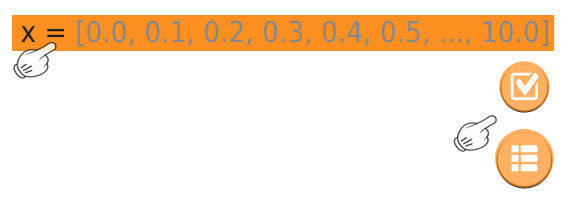
\includegraphics[resolution=320]{how_to_use_fig7.png} \end{tabular}\end{center}

Auch wird ein weiters Action Button
''Details'' angezeigt. Ein Tap auf
diesen Button öffnet das Dialogfenster
''Details'', wo Sie alle Vektorelemente
sehen können.

Bitte beachten Sie, dass die
Verwendung von zwei oder mehr
intervallähnlichen Variablen im linken
Teil einer Ergebnisansicht in dieser
Version des Apps nicht gestattet ist.

\subsection{Funktionsgraph}

Das Funktionsgraph-Element bildet den
Graphen einer Funktion ab, die von
einem einzigen Argument abhängt. Um
einen Graphen zu erstellen, nutzen Sie
den ''Neu'' Button in der Menüleiste
oder ''Funktionsgraph hinzufügen''
Button in der Werkzeugleiste:
\begin{center}\begin{tabular}{c} 
\includegraphics[resolution=320]{how_to_use_fig8.png} \end{tabular}\end{center}

Eine Panel mit sechs lehre Feldern wird
erstellt. Die darzustellenden
Funktionen sollen im linken mittleren
Feld sein und das Funktionsargument im
mittleren unteren Feld.
\begin{center}\begin{tabular}{c} 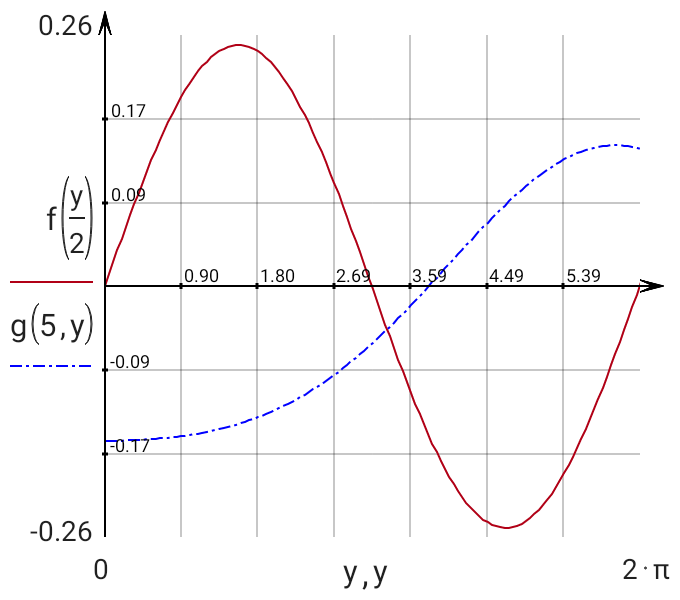
\includegraphics[resolution=320]{how_to_use_fig9.png} \end{tabular}\end{center}

Für mehr Details siehe das ''Plot einer
Funktion'' Beispiel des Hauptmenüs.

\subsection{3D Plot}

Das 3D Plot Element stellt Graphen
einer einzelnen Funktion dar, die von
zwei Argumenten abhängt. Um so einen
Plot zu erstellen, nutzen Sie den
''Neu'' Button in der Menüleiste oder
''3D Plot hinzufügen'' Button in der
Werkzeugleiste:
\begin{center}\begin{tabular}{c} 
\includegraphics[resolution=320]{how_to_use_fig10.png} \end{tabular}\end{center}
\begin{center}\begin{tabular}{cc}
  $x := \left[ -10,\, -9.5 \,..\, 10 \right]$ &
  $y := \left[ -10,\, -9.5 \,..\, 10 \right]$ \cr
\end{tabular}\end{center}
\begin{center}\begin{tabular}{c} 
\includegraphics[resolution=320]{how_to_use_fig11.png} \end{tabular}\end{center}

Fügen Sie im unteren Zentrum den
Funktionsname oder eine Gleichung ein,
die genau zwei zuvor definierte
Intervalle enthält. Sie können hier
auch ein Array benuzen:
\begin{center}\begin{tabular}{c} 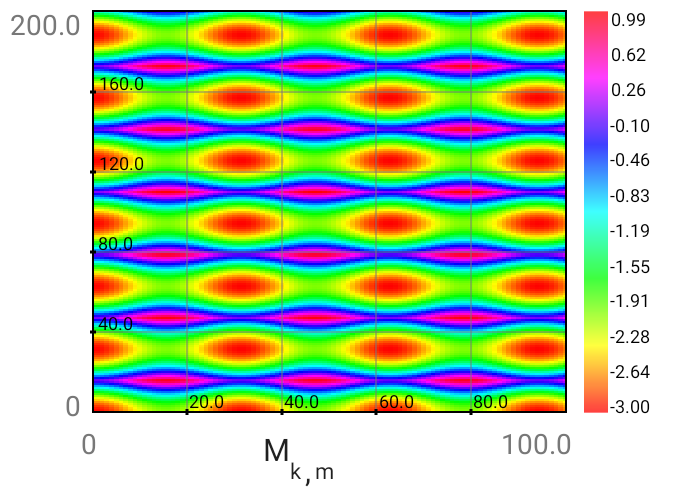
\includegraphics[resolution=320]{how_to_use_fig12.png} \end{tabular}\end{center}

Für mehr Details siehe ''3D Plot''
Beispiel im Hauptmenü.

\subsection{Textfragment}

Das Textfragment Element stellt
einfache Texte wie diesen hier da. Um
ein Textfragment hinzuzufügen, nutzen
Sie den ''Neu'' Button der Menüleiste
oder ''Textfragment hinzufügen'' Button
in der Werkzeugleiste:
\begin{center}\begin{tabular}{c} 
\includegraphics[resolution=320]{how_to_use_fig13.png} \end{tabular}\end{center}

Wenn Sie auf den Text lange gedrückt
halten, und dann den ganzen Text
mittels Kontexmenü  ''Alles auswählen''
markieren,  erscheint ein Action
Button ''Objekteinstellungen''.

Ein Tap auf diesen Button öffnet das
Dialogfenster ''Text-Einstellungen''.
Dort können Sie sowohl Textstil
ändern, als auch  die Numerierung
aktivieren.  Zum Beispiel, die
Überschriften im Dokument haben
Textstil ''Unterabschnitt'' und 
automatische Numerierung.

\subsection{Bild}

Sie können auch ein Bild aus einer
Datei hinzufügen. Nutzen Sie dafür den
Button ''Neu'' in der Menüleiste oder
den Button ''Bild aus Datei hinzufügen''
in der Werkzeugleiste:
\begin{center}\begin{tabular}{c} 
\includegraphics[resolution=320]{how_to_use_fig14.png} \end{tabular}\end{center}

Der Dialog ''Bildeinstellungen'' wird
geöffnet. Dort können Sie eine Datei
auswählen, in der das gewünschte Bild
abgespeichert ist und die gewünschte
Bildgröße festlegen.

Derzeit werden folgende Bildformate
unterstützt: png, bmp, gif, jpeg, svg.

Wenn das Kontrollkästchen ''In Dokument
einbetten'' im Dialog
''Bildeinstellungen'' aktiviert ist,
wird das Bild direkt in Ihr
Arbeitsblatt eingebettet. Das
Arbeitsblatt wird dann größer, kann
aber weiterhin benutzt werden, auch
wenn die ursprüngliche Datei mit dem
Bild gelöscht wurde.

Wenn das Kontrollkästchen ''In Dokument
einbetten'' nicht aktiviert ist, dann
wird das Arbeitsblatt mit dem Bild
verknüpft. Die Verknüpfung ist eine
Referenz auf die Datei außerhalb des
Arbeitsblattes. In diesem Fall müssen
beide Dateien (Arbeitsblatt und
Bilddatei) immer zusammen kopiert oder
verschoben werden.

Die Bildgröße kann mittels des
Dialogfensters ''Bildeinstellungen''
geändert werden. Wenn Sie auf dem Bild
lange gedrückt halten, erscheint ein
Action Button ''Objekteinstellungen''.
Ein Tap auf diesen Button öffnet
dieses Dialogfenster.


\section{Beispiel: Plot einer Funktion}
% This is auto-generated file: do not edit!
% Exported from microMathematics, version 1.18


Dieses Beispiel demonstriert, wie man
die graphische Darstellung einer
Funktion vorbereitet und anpasst.
Nehmen wir an, wir wollen folgende
Funktion aufzeichnen:
\begin{center}\begin{tabular}{c}
  $f(x) := 25 + 10 \cdot sin \left( \sqrt{ \left| x \right| } \right) $
\end{tabular}\end{center}

Das Funktionsargument, das die x-Werte
repräsentiert, wird für N Punkte
innerhalb des Intervalls [x1, x2]
eingesetzt:
\begin{center}\begin{tabular}{ccc}
  $N := 300$ &
  $x1 := -30$ &
  $x2 := 30$ \cr
\end{tabular}\end{center}
\begin{center}\begin{tabular}{c}
  $x := \left[ x1,\, x1 + \left( x2 - x1 \right) / N \,..\, x2 \right]$
\end{tabular}\end{center}

Ist die Funktion und das Argument
definiert, können Sie die Plot Box
hinzufügen indem Sie den ''Neu'' Button
der Menüleiste oder den
''Funktionsgraph hinzufügen'' Button in
der Werkzeugleiste wählen:
\begin{center}\begin{tabular}{c} 
\includegraphics[resolution=320]{graphics/function_plot_fig1.png} \end{tabular}\end{center}
\begin{center}\begin{tabular}{c} 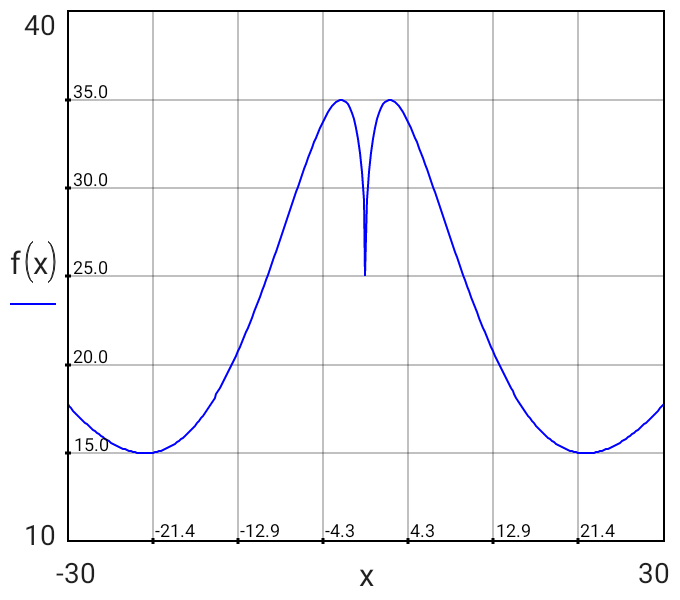
\includegraphics[resolution=320]{graphics/function_plot_fig2.png} \end{tabular}\end{center}

Die darzustellende Funktion soll ins
linke Mittelfeld eingefügt werden. Es
kann ebenfalls eine integrierte oder
zuvor definierte Funktion sein sowie
ein mathematischer Ausdruck, der jeden
anderen Operator oder Funktion
enthalten kann.

Das Funktionsargument, das die x-Werte
repräsentiert, wird in das untere
Mittelfeld eingesetzt. Dies kann eine
Variable eines Intervalltyps oder ein
mathematischer Ausdruck sein, der eine
Intervallvariable enthält.

Die vier anderen Felder definieren die
Plot Grenzen. Falls diese Elemente
leer bleiben, wird das Programm die
entsprechenden Werte automatisch
berechnen. Allerdings können Sie diese
Felder zu jedem Zeitpunkt bearbeiten
und die Werte einsetzten, die Sie
benötigen.

Wenn Sie lange auf die Mitte des Plot
Bereichs drücken, ein Action Button
''Objekteinstellungen'' erscheint:
\begin{center}\begin{tabular}{c} 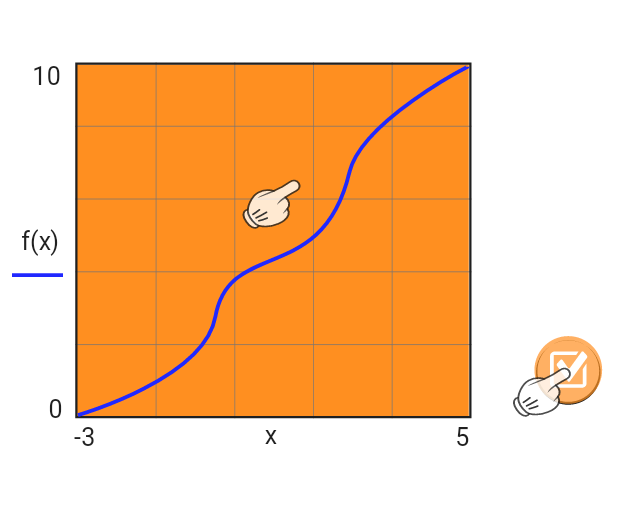
\includegraphics[resolution=320]{graphics/function_plot_fig3.png} \end{tabular}\end{center}

Ein Tap auf diesen Button öffnet das
Dialogfenster ''Plot Einstellungen''.
Hier können die Größe und das Aussehen
des Graphen verändert werden. Ein
verschränkter Graph sieht
beispielsweise so aus:
\begin{center}\begin{tabular}{c} 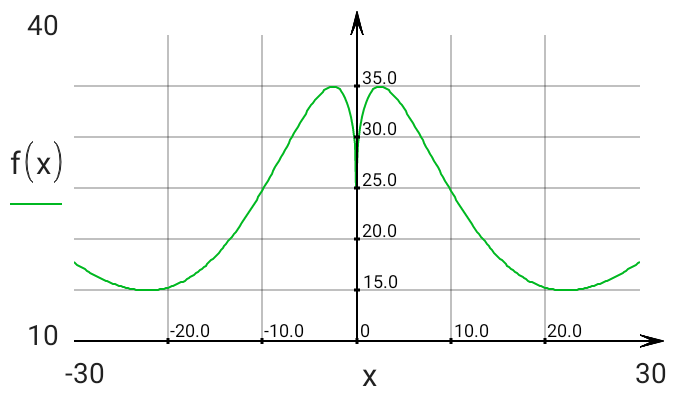
\includegraphics[resolution=320]{graphics/function_plot_fig4.png} \end{tabular}\end{center}

Sie können Strichfarbe, -weite und
-stil im ''Stricheinstellungen'' Dialog
ändern. Es erscheint zudem, wenn Sie
lange auf den grünen Marker unterhalb
des Funktionsnamens auf der linken
Seite des Plot Bereiches drücken:
\begin{center}\begin{tabular}{c} 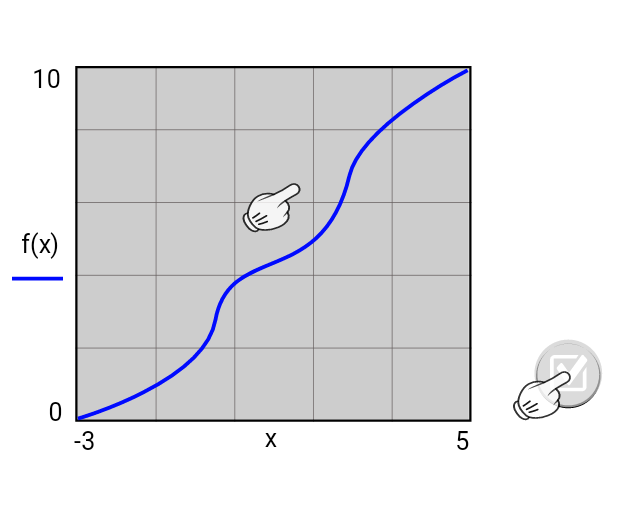
\includegraphics[resolution=320]{graphics/function_plot_fig5.png} \end{tabular}\end{center}

Zum Beispiel, man kann gestrichelte
Linien benutzen:
\begin{center}\begin{tabular}{c} 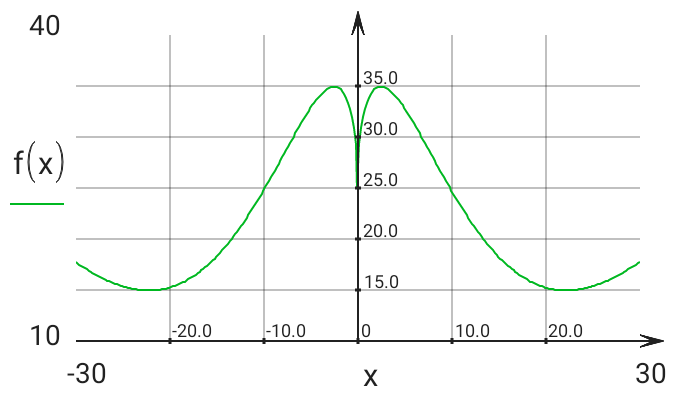
\includegraphics[resolution=320]{graphics/function_plot_fig6.png} \end{tabular}\end{center}

Die Anzahl von Achsenbezeichnungen und
Rasterlinienfarben kann in den
''Rastereinstellungen'' Dialog verändert
werden. Es erscheint, wenn Sie lange
auf den Freiraum zwischen dem
minimalem x-Wert (-30) und dem
Argumentsymbol (x) oder zwischen das
x-Symbol und den maximalen x-Wert (30)
unterhalb des Plot Bereichs drücken:
\begin{center}\begin{tabular}{c} 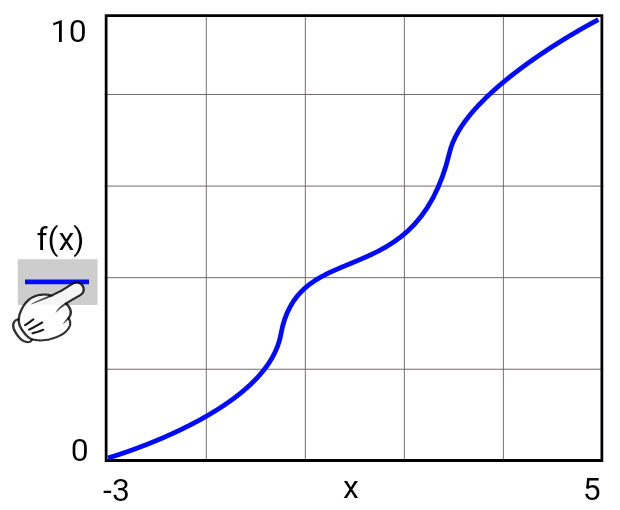
\includegraphics[resolution=320]{graphics/function_plot_fig7.png} \end{tabular}\end{center}
\begin{center}\begin{tabular}{c} 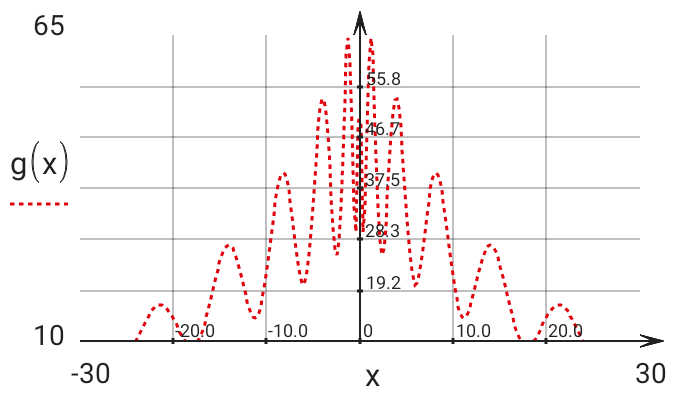
\includegraphics[resolution=320]{graphics/function_plot_fig8.png} \end{tabular}\end{center}

\section{Beispiel: Plot einer Polarfunktion}
% This is auto-generated file: do not edit!
% Exported from microMathematics Plus, version 2.16.1


Jetzt zeichnen wir eine Funktion, die
im Polarkoordinatensystem gegeben ist.
Jeder Punkt in diesem System wird vom
Abstand r zum Ursprung und dem Winkel
f von der x-Achse bestimmt.
\begin{center}\begin{tabular}{c} 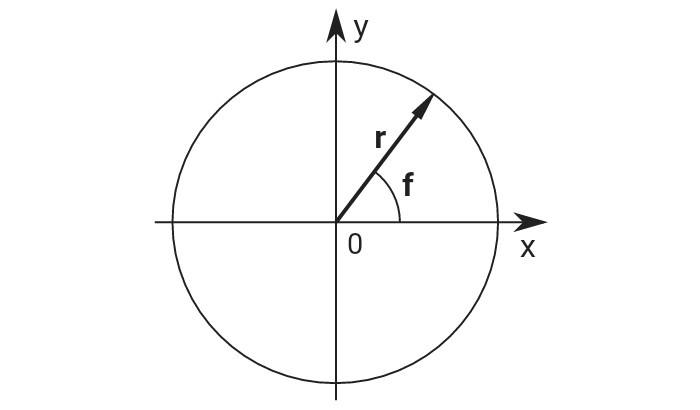
\includegraphics[resolution=320]{graphics/polar_plot_fig1.png} \end{tabular}\end{center}

Der Winkel f ist unsere unabhängige
Variable und wird folgendermaßen
angepasst:
\begin{center}\begin{tabular}{c}
  $f := \left[ 0.01,\, 0.05 \,..\, 300 \right]$
\end{tabular}\end{center}

Der Abstand r(f) ist unsere abhängige
Variable. Mittels des Paares f und r
können wir sie in die kartesischen
Koordinaten x und y umwandeln, indem
wir Sinus- und Kosinus-Funktionen
verwenden:
\begin{center}\begin{tabular}{cc}
  $x(r) := r \cdot cos \left( f\right) $ &
  $y(r) := r \cdot sin \left( f\right) $ \cr
\end{tabular}\end{center}

\subsection{Eine Schnecke}

Wir werden erste Polarfunktion in drei
Schritten definieren. Der erste
Ausdruck definiert ein ''Rad'':
\begin{center}\begin{tabular}{ccc}
  $A := 1.1$ &
  $B := 1.271$ &
  $q := 2$ \cr
\end{tabular}\end{center}
\begin{center}\begin{tabular}{c}
  $r1(f) := A + 2 \cdot {sin \left( B \cdot f\right) }^{q}$
\end{tabular}\end{center}

Um diese Funktion darzustellen, fügen
wir die Plot Box durch den ''Neu''
Button in der Menüleiste oder durch
''Funktionsgraph hinzufügen'' Button in
der Werkzeugleiste hinzu:
\begin{center}\begin{tabular}{c} 
\includegraphics[resolution=320]{graphics/polar_plot_fig2.png} \end{tabular}\end{center}

Anstelle von f und r benutzen wir die
zuvor definierten Regeln für
Umwandlungen von x und y, wobei rl(f)
als ein symbolisches Argument für
diese Regeln eingesetzt wird:
\begin{center}\begin{tabular}{c} 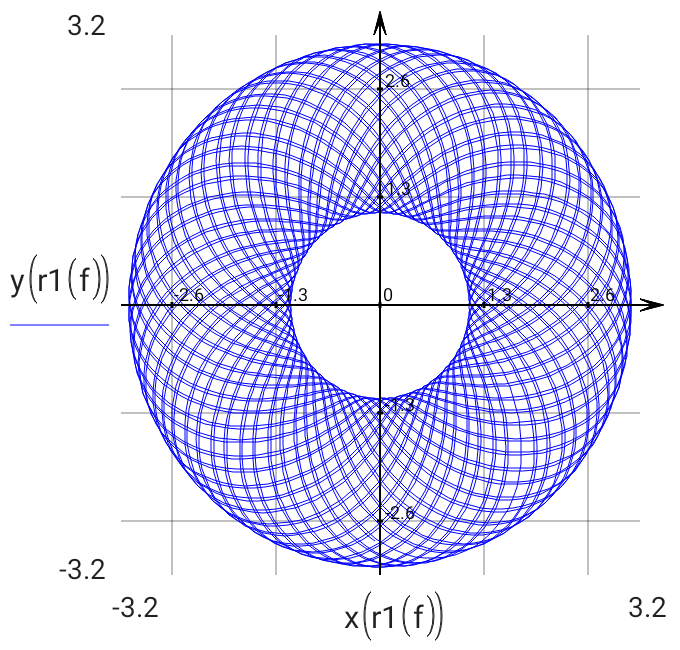
\includegraphics[resolution=320]{graphics/polar_plot_fig3.png} \end{tabular}\end{center}

Als nächstes können wir dieses Rad wie
folgt modifizieren:
\begin{center}\begin{tabular}{c}
  $r2(f) := A + 2 \cdot {sin \left( B \cdot f + 1 \cdot r1 \left( f\right) \right) }^{q}$
\end{tabular}\end{center}
\begin{center}\begin{tabular}{c} 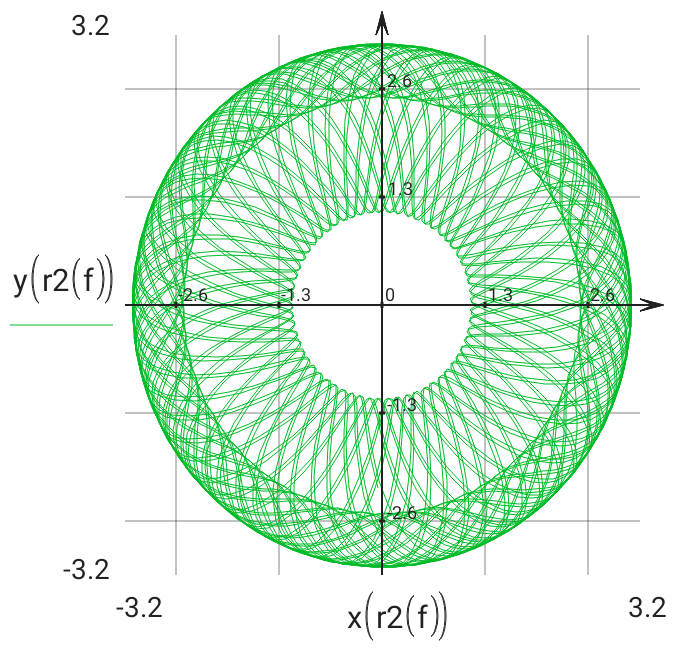
\includegraphics[resolution=320]{graphics/polar_plot_fig4.png} \end{tabular}\end{center}

Abschließend skalieren wir die letzte
Funktion r2(f), indem wir eine
Abrundung auf die nächstniedrigere
Ganzzahl verwenden, was wie eine
Stufenfunktion aussieht. Als Ergebnis
erhalten wir eine schöne Schnecke:
\begin{center}\begin{tabular}{c}
  $r(f) := r2 \left( f\right)  \cdot floor \left( f\right)  / 10$
\end{tabular}\end{center}
\begin{center}\begin{tabular}{c} 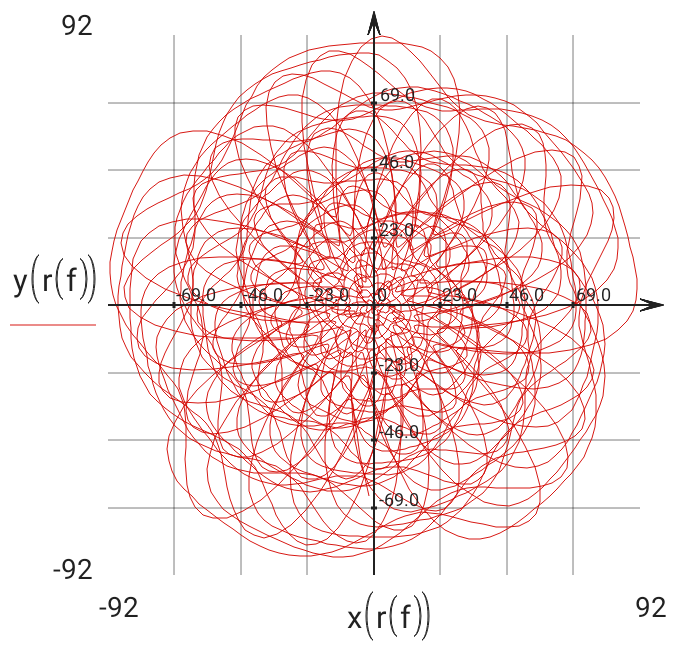
\includegraphics[resolution=320]{graphics/polar_plot_fig5.png} \end{tabular}\end{center}

\subsection{Japanischer Ahorn}

Japanischer Ahorn ist bekannt für die
schönen Formen und Farben seiner
Blätter. Solch ein Blatt kann
mathematisch beschrieben werden und
als Kurve im Polarkoordinatensystem
dargestellt werden:
\begin{center}\begin{tabular}{c}
  $f := \left[ 0.01,\, 0.02 \,..\, 100 \right]$
\end{tabular}\end{center}
\begin{center}\begin{tabular}{cc}
  $x(r) := r \cdot cos \left( f\right) $ &
  $y(r) := r \cdot sin \left( f\right) $ \cr
\end{tabular}\end{center}
\begin{center}\begin{tabular}{c}
  $s1(f) := \left( 1 + sin \left( f\right)  \right) \cdot \left( 1 - 0.9 \cdot  \left| sin \left( 4 \cdot f\right)  \right|  \right)$
\end{tabular}\end{center}
\begin{center}\begin{tabular}{c}
  $s2(f) := 0.9 + 0.05 \cdot cos \left( 200 \cdot f\right) $
\end{tabular}\end{center}
\begin{center}\begin{tabular}{c}
  $r(f) := floor \left( f\right)  \cdot s1 \left( f\right)  \cdot s2 \left( f\right)  + random \left( 2\right)  - 1$
\end{tabular}\end{center}
\begin{center}\begin{tabular}{c} 
\includegraphics[resolution=320]{graphics/polar_plot_fig6.png} \end{tabular}\end{center}

http://en.wikipedia.org/wiki/Acer\_palmatum

\section{Beispiel: 3D Plot}
% This is auto-generated file: do not edit!
% Exported from microMathematics Plus, version 2.17.1


Dieses Beispiel demonstriert 3D Plots
zu drei verschiedenen Funktionen
zweier Variablen.

Zuerst definieren wir Intervalle für
x- und y-Argumente. Das Intervall der
x-Achse hängt von der Anzahl der
Punkte entlang der x-Achse sowie den
Minimal- und Maximalwerten x1 und x2
ab:
\begin{center}\begin{tabular}{ccc}
  $N := 300$ &
  $x1 := -2$ &
  $x2 := 2$ \cr
\end{tabular}\end{center}
\begin{center}\begin{tabular}{c}
  $x := \left[ x1,\, x1 +  \left| x2 - x1 \right|  / N \,..\, x2 \right]$
\end{tabular}\end{center}

Das Intervall für die y-Achse wird dem
entsprechend definiert:
\begin{center}\begin{tabular}{ccc}
  $M := 300$ &
  $y1 := -3$ &
  $y2 := 3$ \cr
\end{tabular}\end{center}
\begin{center}\begin{tabular}{c}
  $y := \left[ y1,\, y1 +  \left| y2 - y1 \right|  / M \,..\, y2 \right]$
\end{tabular}\end{center}

Wir zeichnen nun als Beispiel eine
trigonometrische Funktion, die ein
Produkt von Sinus und Kosinus ist:
\begin{center}\begin{tabular}{c}
  $F(x,y) := sin \left( 3 \cdot {x}^{2}\right)  \cdot cos \left( {y}^{2}\right) $
\end{tabular}\end{center}

Für die 3D Ansicht klicken Sie auf ''3D
Plot hinzufügen'' in der Werkzeugleiste
oder ''Neu'' in der Menüleiste:
\begin{center}\begin{tabular}{c} 
\includegraphics[resolution=320]{graphics/three_d_plot_fig1.png} \end{tabular}\end{center}

Setzen Sie den Funktionsnamen F(x,y) in
das untere Mittelfeld:
\begin{center}\begin{tabular}{c} 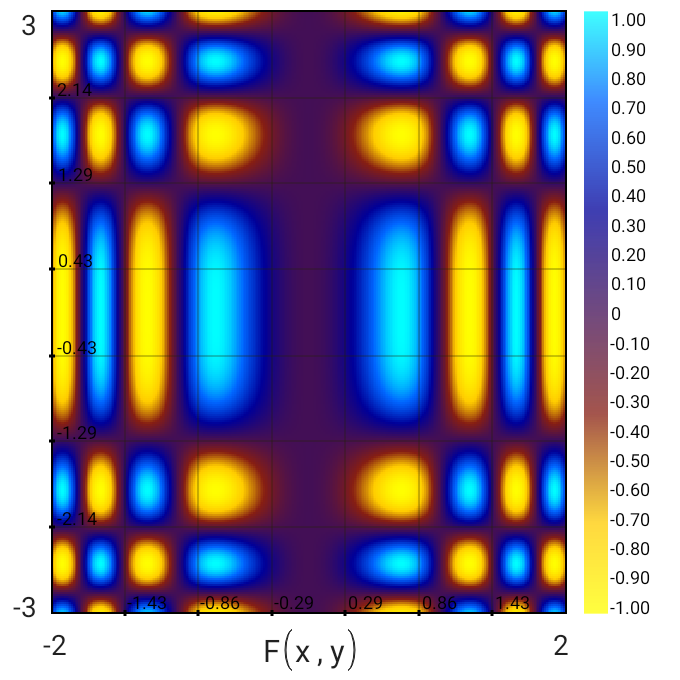
\includegraphics[resolution=320]{graphics/three_d_plot_fig2.png} \end{tabular}\end{center}

Plot Grenzen, Größe, Stil, Bezeichnung
und Raster können mittels des
Dialogfensters ''Plot Einstellungen''
angepasst werden (siehe das Beispiel
zu ''Plot einer Funktion'' im Hauptmenü
für mehr Informationen). Wenn Sie auf
die Mitte des Plot Bereichs lange
gedrückt halten, erscheint ein Action
Button ''Objekteinstellungen''. Ein Tap
auf diesen Button öffnet dieses
Dialogfenster.

Zudem können Sie die Anzahl der
Bezeichnungen entlang der z-Achse
ändern und die Farbenpalette im Dialog
''Farbtabellen Einstellungen'' wählen.
Dieser Dialog erscheint ebenfalls
durch langes Drücken der z-Achse im
rechten Bereich des Hauptgraphen.
\begin{center}\begin{tabular}{c}
  $R(x,y) := sin \left( 5 \cdot {x}^{2} \cdot \left( y - x \right)\right) $
\end{tabular}\end{center}
\begin{center}\begin{tabular}{c} 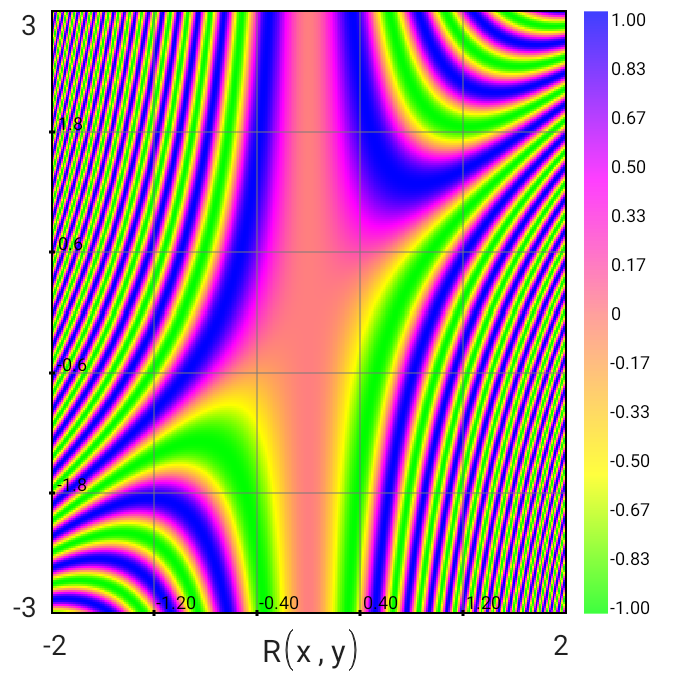
\includegraphics[resolution=320]{graphics/three_d_plot_fig3.png} \end{tabular}\end{center}

Eine Funktion zweier Argumente kann
ebenso als Oberfläche im
dreidimensionalen Raum aufgetragen
werden. Dieser Modus kann in den ''Plot
Einstellungen'' Dialog aktiviert
werden, indem man den Button
''Objekteinstellungen'' clickt, der
durch langes Gedrückthalten auf die
Mitte des Plot Bereichs erscheint. Um
die Berechnungszeit zu verbessern,
verwenden wir Arrays und zeichnen nun
die folgende Funktion F(n,m):
\begin{center}\begin{tabular}{cccc}
  $N := 100$ &
  $n := \left[ 0,\, 1 \,..\, N \right]$ &
  $x1 := -15$ &
  $x2 := 15$ \cr
\end{tabular}\end{center}
\begin{center}\begin{tabular}{cccc}
  $M := 100$ &
  $m := \left[ 0,\, 1 \,..\, M \right]$ &
  $y1 := -15$ &
  $y2 := 15$ \cr
\end{tabular}\end{center}
\begin{center}\begin{tabular}{c}
  $x[n] := {\left( x1 +  \left( x2 - x1\right)  \cdot n / N \right)}^{2}$
\end{tabular}\end{center}
\begin{center}\begin{tabular}{c}
  $y[m] := {\left( y1 +  \left( y2 - y1\right)  \cdot m / M \right)}^{2}$
\end{tabular}\end{center}
\begin{center}\begin{tabular}{c}
  $r[n,m] := 0.04 \cdot x_{n}  + 0.02 \cdot y_{m} $
\end{tabular}\end{center}
\begin{center}\begin{tabular}{c}
  $t[n,m] := \left( x_{n}  + 0.05 \cdot y_{m}  \right) \cdot exp \left( 1 - r_{n,\, m} \right) $
\end{tabular}\end{center}
\begin{center}\begin{tabular}{c}
  $F[n,m] := \frac{sin \left( x_{n}  + 0.1 \cdot y_{m} \right) }{0.15 + r_{n,\, m} } + \frac{t_{n,\, m} }{10}$
\end{tabular}\end{center}
\begin{center}\begin{tabular}{c} 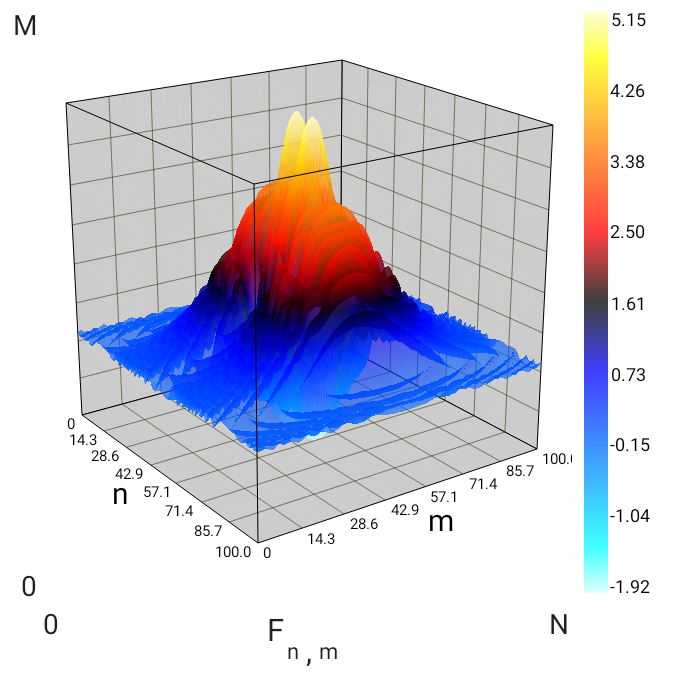
\includegraphics[resolution=320]{graphics/three_d_plot_fig4.png} \end{tabular}\end{center}

Um die Plot Oberfläche zu gestalten
gibt es zusätzliche Einstellungen, die
im Dialog ''Plot Einstellungen'' zu
finden sind. Sie können wählen, ob die
Netzlinien sichtbar sein sollen,
welche Deckkraft deren Farbe haben
soll, oder die Rotations- und
Elevationswinkel der Plot Box
definieren. Zum Beispiel, die oben
gezeigte Oberfläche sieht aus der
anderen Perspektive so aus: 
\begin{center}\begin{tabular}{c} 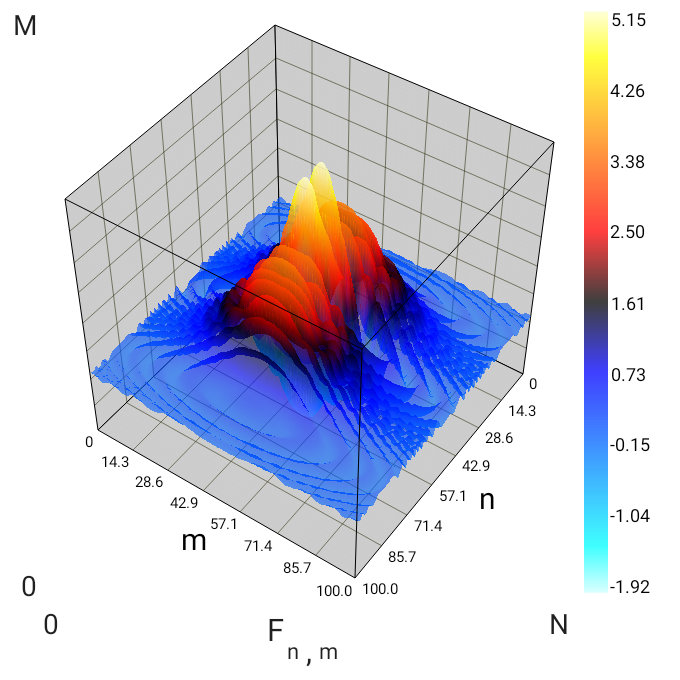
\includegraphics[resolution=320]{graphics/three_d_plot_fig5.png} \end{tabular}\end{center}

\section{Beispiel: Reihen und Integrale}
% This is auto-generated file: do not edit!
% Exported from microMathematics Plus, version 2.15.6


Dieses Beispiel zeigt, wie Sie Reihen
und Integrale berechnen können.

\subsection{Taylor Reihe}

In der Mathematik ist die Taylor Reihe
eine Repräsentation einer Funktion als
unendliche Summe von Termen, die von
den Werten der Ableitung dieser
Funktion an einem bestimmten Punk
berechnet werden.

Beispielsweise ist Ts(x,N) die
Taylorentwicklung als Funktion des
Arguments x und der Anzahl von N
Termen:
\begin{center}\begin{tabular}{c}
  $Ts(x,N) := \displaystyle\sum_{n=0}^{N} \frac{{ \left( -1\right) }^{n}}{\left( 2 \cdot n \right)! } \cdot {x}^{2 \cdot n}$
\end{tabular}\end{center}

Diese Entwicklung nähert sich der
Kosinus-Funktion an:
\begin{center}\begin{tabular}{c}
  $s(x) := cos \left( x\right) $
\end{tabular}\end{center}

Wenn wir beide Funktionen für das selbe
Intervall auftragen, so sehen beide
gleich aus: 
\begin{center}\begin{tabular}{c}
  $x := \left[ 0,\, 0.1 \,..\, 2 \cdot {\pi} \right]$
\end{tabular}\end{center}
\begin{center}\begin{tabular}{c} 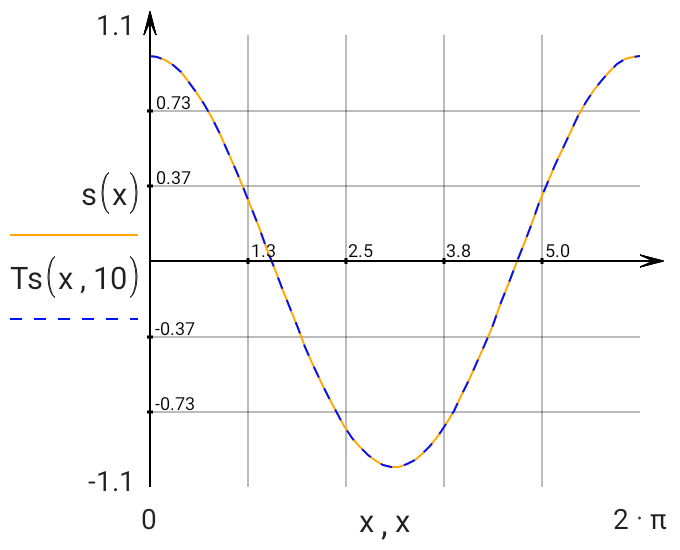
\includegraphics[resolution=320]{graphics/series_and_integrals_fig1.png} \end{tabular}\end{center}

Jedoch ist dies ein numerischer Fehler,
der aus der eingeschränkten Anzahl von
Annäherungstermen N resultiert. Die
folgende Funktion $\Delta$(x,N) beschreibt
diesen Fehler:
\begin{center}\begin{tabular}{c}
  ${\Delta}(x,N) :=  \left| s \left( x\right)  - Ts \left( x,\, N\right)  \right| $
\end{tabular}\end{center}

Wir können diese Funktion in
logarithmischen Koordinaten ausdrücken
und werden sehen, dass der numerische
Fehler sich verringert hat, wenn wir
mehr Terme in die Taylorreihe
integrieren:
\begin{center}\begin{tabular}{c}
  $E(N) := log10 \left( {\Delta} \left( {\pi},\, N\right) \right) $
\end{tabular}\end{center}
\begin{center}\begin{tabular}{c}
  $N := \left[ 3,\, 4 \,..\, 13 \right]$
\end{tabular}\end{center}
\begin{center}\begin{tabular}{c} 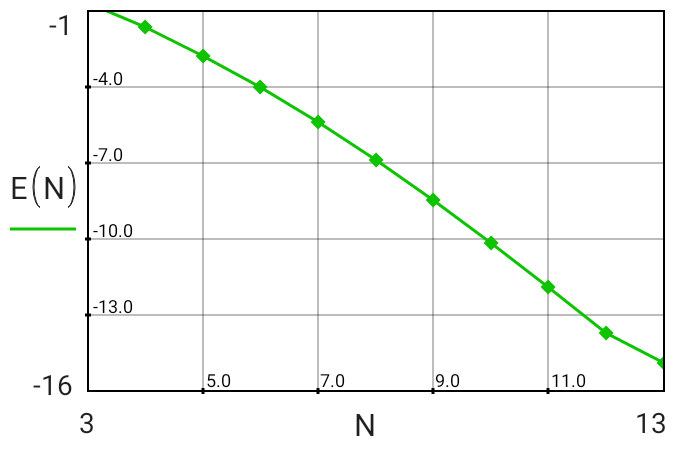
\includegraphics[resolution=320]{graphics/series_and_integrals_fig2.png} \end{tabular}\end{center}

\subsection{Binomische Reihen}

Betrachten wir diese Potenzfunktion:
\begin{center}\begin{tabular}{c}
  $f(x,{\alpha}) := {\left( 1 + x \right)}^{{\alpha}}$
\end{tabular}\end{center}

Dieser Funktion kann sich durch eine
Binomische Reihe angenähert werden:
\begin{center}\begin{tabular}{c}
  $Tf(x,{\alpha},N) := \displaystyle\sum_{n=0}^{N}  \left( \displaystyle\prod_{k=1}^{n} \frac{{\alpha} - k + 1}{k}\right)  \cdot {x}^{n}$
\end{tabular}\end{center}

Zudem können wir beide Funktionen (die
gegebene Potenzfunktion und ihre
Annäherung) im gleichen Plot
auftragen:
\begin{center}\begin{tabular}{c} 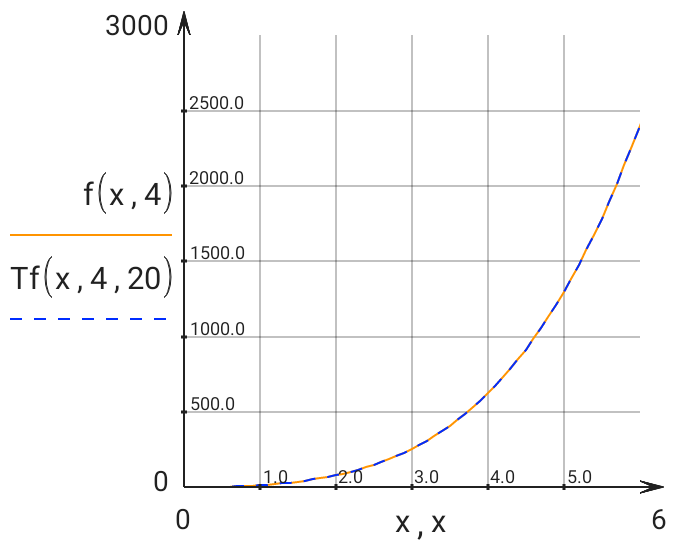
\includegraphics[resolution=320]{graphics/series_and_integrals_fig3.png} \end{tabular}\end{center}

\subsection{Integrale}

Außerdem ist es möglich, ein
bestimmtes Integral mittels der
Simpson Methode numerisch zu
berechnen. Beispielsweise können wir
das Integral durch das Element
''Ergebnisansicht'' berechnen:
\begin{center}\begin{tabular}{c}
  $\displaystyle\int_{0}^{3 \cdot pi / 2}{cos \left( \frac{2 \cdot x}{9}\right) }^{-2}\, dx = 7.79423$
\end{tabular}\end{center}

Das analytische Ergebnis ist
\begin{center}\begin{tabular}{ccc}
  $I := \frac{9 \cdot \sqrt{3} }{2}$ &
  ,    &
  $I = 7.79423$ \cr
\end{tabular}\end{center}

Der numerische Fehler kann wie folgt
berechnet werden:
\begin{center}\begin{tabular}{c}
  $\displaystyle\int_{0}^{3 \cdot pi / 2}{cos \left( \frac{2 \cdot x}{9}\right) }^{-2}\, dx - I = 4.26681E-9$
\end{tabular}\end{center}

Dieser Fehler hängt von dem Wert
''Signifikante Ziffern im Ergebnis'' ab,
was in den ''Dokumenteinstellungen''
Dialog verändert werden kann:
\begin{center}\begin{tabular}{c} 
\includegraphics[resolution=320]{graphics/series_and_integrals_fig4.png} \end{tabular}\end{center}

Wird dieser Wert erhöht, so erhöht sich
auch die Grenze, welche die
Genauigkeit der Simpson Methode
kontrolliert.

\section{Info zu microMathematics Plus}

% This is the second part of the file about_micromath_de.tex
\subsection{Autoren}

\begin{enumerate}
\item Mikhail Kulesh,
mikhail.kulesh@gmail.com

\item Caio Roberto Ramos da Silva
(Übersetzung auf brasilianisches
Portugiesisch),
caiorrs@gmail.com
\end{enumerate}

\subsection{Das App Icon}

Das App Icon ist generiert mit Hilfe
folgender Funktion, die im
Polarkoordinatensystem gegeben ist:
\begin{center}\begin{tabular}{c}
  $f := \left[ 0.01,\, 0.03 \,..\, 150 \right]$
\end{tabular}\end{center}
\begin{center}\begin{tabular}{c}
  $s(f) := 4 + sin \left( 5 \cdot f\right)  + \frac{sin \left( 10 \cdot f\right) }{2} + \frac{sin \left( 60 \cdot f\right) }{6}$
\end{tabular}\end{center}
\begin{center}\begin{tabular}{c}
  $r(f) := 0.9 \cdot \left( 1 + f / 50 \right) \cdot s \left( f\right) $
\end{tabular}\end{center}
\begin{center}\begin{tabular}{c}
  $x(f) := r \left( f\right)  \cdot cos \left( f\right) $
\end{tabular}\end{center}
\begin{center}\begin{tabular}{c}
  $y(f) := r \left( f\right)  \cdot sin \left( f\right) $
\end{tabular}\end{center}
\begin{center}\begin{tabular}{c} 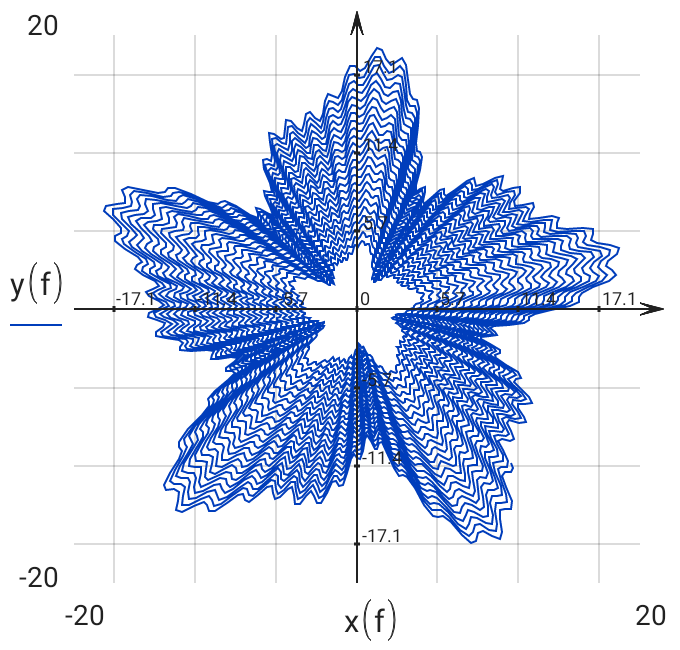
\includegraphics[resolution=320]{graphics/about_micromath_fig1.png} \end{tabular}\end{center}

2014-2017, Bremen, Deutschland
\end{document}
